%Review of timbral control research.
%	Timbre Definition
%	Timbre Spaces (MDS and shit)
%	Audio Features
%	Perceptual Control of Synthesis

\chapter{Timbre}
\label{chap:Timbre}
\note
{
	CataRT system developed by \citet{schwarz2007corpus}.

	Temporal features, hidden markov models to look at feature change over time. 

	All that stuff about only distorting the only the sustain.

	Timbral effects of amplitude envelope being reversed \citep{patterson1994the}.

}

\section{Introduction}
\label{sec:Timbre-Introduction}
	There are three properties which describe how a sound is perceived, these being loudness, pitch and timbre. Loudness
	describes the perceived intensity of a sound and pitch its perceived frequency. Timbre then describes any other
	properties of a sound, besides loudness and pitch, which allow it to be distinguished from other sounds
	\citep{mathews1999introduction}. Loudness and pitch are both one dimensional properties allowing sounds to be
	ordered from quiet to loud or low to high pitch. Timbre is a more complex property consisting of multiple dimensions
	\citep{rossing2002the}. There is a large body of research concerning the analysis of timbre, identifying these
	dimensions and their relationships with the acoustic features of a sound.

	\note
	{
		better introduce this paragraph (layman's description)
	}

	Simple descriptions of a sounds timbre involve instrument identification. A sound could be described as `cello-like'
	or `flute-like'. More broadly the class of instrument, string or woodwind, could be used to describe the timbre of a
	sound. While these terms are useful for discussing the instrumentation of pieces they can not be applied generally
	to a wide range of timbres. It is not very useful to describe the timbre of a xylophone as being `not flute-like'.

	More general timbral descriptors directly describe the sound itself rather than the source which produced it. These
	include terms such as bright, rough and sharp. This allows the timbre of different sounds to be compared according
	to these terms \citep{howard2009acoustics}. Sounds can also be ordered in respect to these criteria much like with
	loudness and pitch. For example one could order a set of sounds by how bright they sound.

	Early research into timbre was performed by \citet{helmholtz1875on}. More recent work involves research from various
	fields. Low level features of audio segments can be found using signal analysis techniques. More complicated
	information about the perception of a signal can be discovered through modelling the behaviour of the human hearing
	system. Lastly experiments can be undertaken in which participants listen to audio samples and provide responses
	regarding the timbre of the samples. These responses are then analysed to uncover any correlations between the
	participants responses and lower level features of the audio samples.

	This chapter will review the existing body of timbral research. Section \ref{sec:Timbre-LowLevelFeatures} discusses
	metric which are used to describe the low level features of audio signals. Section
	\ref{sec:Timbre-PsychoacousticPrinciples} covers various models which describe the perception of various auditory
	phenomena. \note{Put in what the rest of the sections are about}.

	\note
	{
		discuss where the current vocabulary comes from and the general world of timbre description

		discuss state of the art and where this thesis takes on from that
	}

\section{Low Level Audio Features}
\label{sec:Timbre-LowLevelFeatures}
	A widely cited definition of timbre \citep{ASA1960american} suggests that timbre in influenced by various low level
	features of an audio signal. The spectral content, waveform and temporal characteristics all effect the perceived
	timbre of a sound. Signal analysis techniques can be used to extract information about these elements of a signal.
	A large list of such feature extraction techniques is given by \citep{peeters2004a}. These features can be
	separated into three categories. Features which describe the properties of a signals waveform and how it evolves
	with time (temporal features), features which describe the frequency content of a signal (spectral features) and
	features which describe how the frequency content of a signal evolves with time (spectro-temporal features). 

	\subsection{Temporal Features}
	\label{sec:Timbre-LowLevelFeatures-Temporal}
		Simple temporal features involve taking statistical measurements, such as mean and variance, of the audio
		samples in a signal. These measures give basic information about the level and variation in a signal but in
		many cases they do not represent a signals properties very well. For example, the mean value of a sinusoidal
		signal over a whole number of cycles is zero. 

		A common technique to extract more meaningful information about a signals level is to use an envelope
		detector. An envelope detector extracts the amplitude envelope of a signal. The amplitude envelope provides
		information about the level of a signal over time. An example amplitude envelope is shown in Figure
		\ref{fig:AmplitudeEnvelope}.

		\begin{figure}[h!]
			\centering
			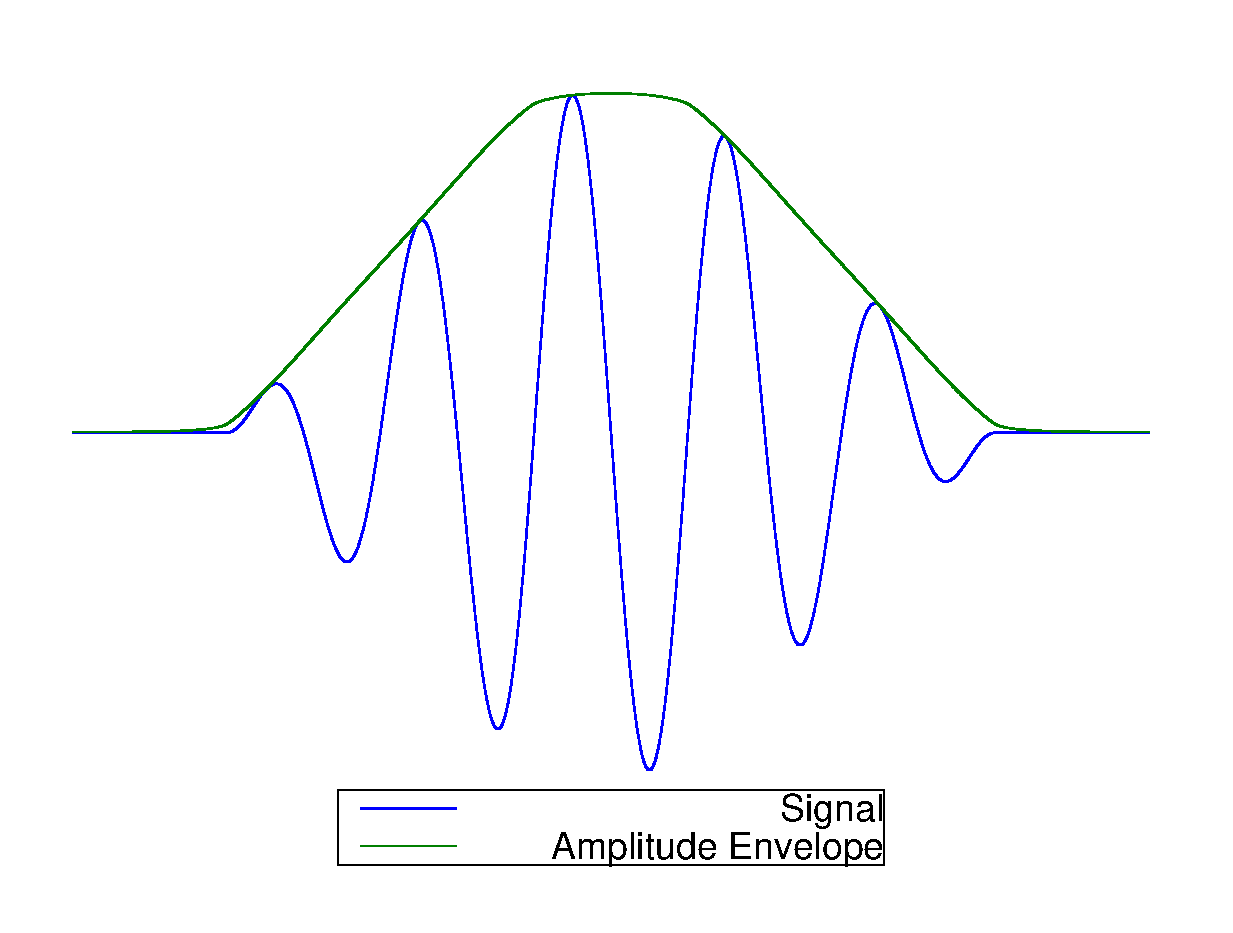
\includegraphics[width=0.6\textwidth]{chapter2/Images/AmplitudeEnvelope.eps}
			\caption{The Amplitude Envelope of a Signal.}
			\label{fig:AmplitudeEnvelope}
		\end{figure}

		Various envelope detection methods are reviewed by \citet{chang2007a}. \citet{howard2009acoustics} separates
		the envelope of a sound into three sections. The steady state section is the middle portion in which the
		timbre of the sound only varies slightly. The onset and offset sections describe the way the sound rises
		from silence to the steady state and returns to silence after. Further refinement of the description of
		amplitude envelopes leads to the ADSR (Attack, Decay, Sustain, Release) model \citep{descrivan2012music}. An
		example ADSR envelope is shown in Figure \ref{fig:ADSR}.

		\begin{figure}[h!]
			\centering
			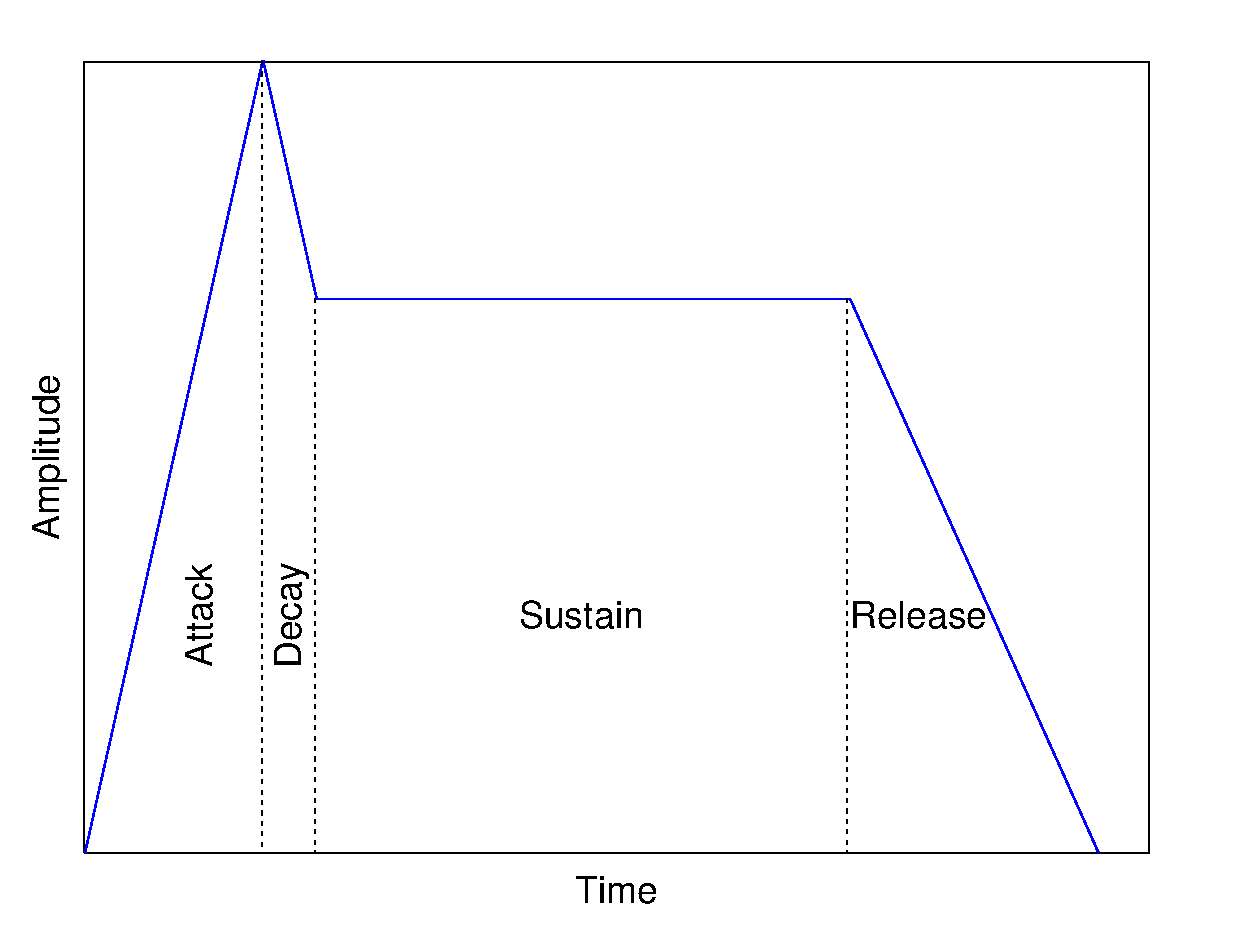
\includegraphics[width=0.6\textwidth]{chapter2/Images/ADSR.eps}
			\caption{An ADSR Envelope.}
			\label{fig:ADSR}
		\end{figure}

		Once the amplitude envelope of a signal has been extracted further statistics can be calculated from it such
		as log attack time and temporal centroid \citep{peeters2000instrument}.

		Some other temporal features measure the oscillation or repetition of a signal. Examples are the zeros
		crossing rate and the autocorrelation, both of which can be used in pitch / frequency estimation
		\citep{mcleod2005a}.

		\note
		{
			pmf features as used by \citet{wilson2014profiling}
		}

	\subsection{Spectral Features}
	\label{sec:Timbre-LowLevelFeatures-Spectral}
		In existing timbral research is is widely reported that features of a sounds spectrum produce the largest
		effects on timbre. Simple spectral features can be calculated as statistical measures which describe the
		shape of the spectrum. For example the spectral centroid of a signal is calculated as the mean frequency
		weighted by their magnitudes. Spectral centroid is often stated as being one of the most salient audio
		features in timbre recognition \citep{freed1990auditory, lakatos2000a}. Higher order statistical moments of
		the spectrum (standard deviation, skewness and kurtosis) can be used to further describe the distribution of
		energy in the spectrum around the centroid.

		More detailed metrics in the shape of a spectrum can be calculated in the form of Mel Frequency Cepstral
		Coefficients (MFCCs). These measurements were originally used in speech recognition systems
		\citep{davis1980comparison}. More recently they have been applied to the analysis of timbre
		\citep{depoli1997sonological}. 

		Other spectral metrics consider the harmonic structure of a signal. In order to calculate these features the
		partials (prominent frequency components) of the signal must me found. The deviation of these partials from
		perfect harmonic frequencies measures the inharmonicity of the signal. \citet{fletcher1962quality} state
		that inharmonicity of some partials is necessary for the recognition of the timbre of a piano. The noise
		energy in a signal describes any energy which is does not contribute to a partial. The noisiness is then
		measured as the ratio of the noise energy to the total energy in the signal \citep{serra1998sound}.

		Further analysis can be performed by finding the harmonic partials of the signal. In detecting the harmonic
		partials it is usual to allow for a slight deviation from perfect harmonic structure, as described by
		\citet{peeters2011the}. Several metrics have been suggested which constitute the ratio of energy between two
		different sets of harmonic partials. The tristimulus metrics proposed by \citet{pollard1982a} split the
		harmonic series in to three sections, the fundamental frequency, the second through fourth harmonics and,
		the rest of the higher order harmonics. Ratios between each of these sections and the total energy in all
		the harmonics are calculated. Another commonly used metric is the ratio between energy in the odd and even
		order harmonic partials. This was found to be a salient feature in the judgement of timbre dissimilarity by
		\citet{hall2010importance}. 

		\note
		{
			Spectro-temporal features exist such as spectral flux.
		}

\section{Psychoacoustic Principles}
\label{sec:Timbre-PsychoacousticPrinciples}
	Psychoacoustics is a field which deals with the perception of sound. The existing literature concerns the study of
	the human hearing system and how it responds to certain aspects of audio stimuli. Several different areas of audio
	perception have been researched. Methods have been devised to model the human perception of loudness
	\citep{moore1997a} and pitch \citep{gerhard2003pitch}. Other research considers the human hearing systems ability to
	locate sound sources \citep{blauert1997spatial}. 

	As discussed in Section \ref{sec:Timbre-LowLevelFeatures-Spectral} there are several metrics to describe the
	spectral content of a signal. While it may be possible to measure changes in values of these features, the changes
	may not be detectable by the human hearing system. Psychoacoustic models allow us to determine how audio signals are
	interpreted by the human hearing system and how well we will notice such changes.

	\subsection{Critical Bands}
	\label{sec:Timbre-PsychoacousticPrinciples-CriticalBands}
		The part of the inner ear which deals with frequency separation is know as the basilar membrane. This is a
		structure which resonates at different frequencies along its length. Low frequencies at one end to high at
		the other. A sinusoidal tone excites a portion of the basilar membrane corresponding to a narrow band of
		frequencies. Two tones whose excitation bands overlap will interfere with how each other are perceived by
		the listener.

		The basilar membrane can be modelled as a filter bank comprised of band pass filters. Each of these
		auditory filters represents the region of the membrane excited by a sinusoidal tone at its centre
		frequency. The bandwidth of these filters is known as the critical bandwidth. Portions of signals will
		interfere with the perception of others which are within one critical bandwidth.
		\citet{glasberg1990derivation} simplify the auditory filters by modelling them as rectangular filters. The
		bandwidth of these filters known as the equivalent rectangular bandwidth (ERB) and can be approximated using
		Equation \ref{eq:ERB}.

		\begin{equation}
			\textrm{ERB}(f_{c}) = 24.7(4.37f_{c} + 1)
			\label{eq:ERB}
		\end{equation}

		Where $f_{c}$ is the center frequency of the auditory filter in kHz and ERB$(f_{c})$ is the equivalent
		rectangular bandwidth, in Hz, at that frequency.

		\citet{howard2009acoustics} discusses the perception of two tones, sounded simultaneously, as they get
		further apart in frequency. When within 15Hz of one another the two tones are perceived as a single sound
		with a sinusoidally varying amplitude. The frequency of this variation is equal to the difference in
		frequency of the tones. As the difference in frequencies gets greater then 15Hz this amplitude modulation
		becomes fast enough for it to be perceived as a roughness in texture rather than `beats' in the amplitude.
		In between 15Hz and the critical bandwidth the perceived sound transitions from a single sound to two
		separate sounds but still with a rough texture. Once the difference in frequencies exceeds the critical
		bandwidth the two tones are perceived as separate smooth tones. These effects are summarised in Figure
		\ref{fig:ToneSeparation}.

		\begin{figure}[h!]
			\centering
			\begin{tikzpicture}

				\draw [thick, ->] (0, 0) -- (10, 0);
				\draw (0, 1) -- (10, 1);
				\draw (0, 0) -- (0, 2) -- (10, 2);

				\draw (0, 0) -- (0, -2pt) node [anchor=north] {0};
				\draw (2, 0) -- (2, -2pt) node [anchor=north] {15};
				\draw (8, 0) -- (8, -2pt) node [anchor=north] {CB};

				\fill [pattern=north west lines] (1.75, 0) rectangle (2.25, 1);
				\fill [pattern=north west lines] (7.75, 0) rectangle (8.25, 1);
				\fill [pattern=north west lines] (5.75, 1) rectangle (6.25, 2);

				\node at (0.875, 0.5) {Beats};
				\node at (5, 0.5) {Rough};
				\node at (9.125, 0.5) {Smooth};
				\node at (2.875, 1.5) {Fused};
				\node at (8.125, 1.5) {Separate};

				\node at (5, -1) {Frequency Difference (Hz)};

			\end{tikzpicture}
			\caption{The perceived of two tones as they move further apart in frequency. Hashed areas represent
				 the transition between perceived effects. CB denotes the critical bandwidth.}
			\label{fig:ToneSeparation}
		\end{figure}

		It is evident from Equation \ref{eq:ERB} that the critical bandwidth increases with frequency. This together
		with the perceptual information shown in Figure \ref{fig:ToneSeparation} suggests that tones separated by
		the same amount will be heard as separate if they or both low in frequency but as their frequencies rise
		they will start to be perceived as a single fused sound.

	\subsection{Specific Loudness}
	\label{sec:Timbre-PsychoacousticPrinciples-SpecificLoudness}
		In hearing models for measuring loudness it is common to split the audible spectrum into bands which all
		have the same perceived width. Before calculating the total loudness the specific loudness for each of these
		bands is calculated. The procedure for doing this is beyond the scope of this report. A description of this
		process is provided by \citet{moore1997a}. The specific loudness measures the perceived loudness of a signal
		in a given frequency range. For the analysis of the perception of timbre this allows for better modelling of
		what portions of a signals spectrum are audible. While the spectrum describes what frequency content is
		present in the signal, the specific loudness describes how much of each frequency is perceived by a
		listener.

		A widely used set of bands was proposed by \citet{zwicker1961subdivision} who spilt the spectrum into 24
		bands, each one critical bandwidth wide. These bands are known and the bark bands and provide a perceptual
		unit of frequency, the bark. Integer values of barks occur at the boundaries between two bark bands. An
		change in frequency of one bark is equal to one critical bandwidth.

	\note
	{
		Perhaps some more on masking. Although it may be wasted space.
	}

\section{Timbral Features}
\label{sec:Timbre-TimbralFeatures}
	Models have been developed in the literature to describe certain aspects of the timbre of a sound. Two such models
	are those for describing auditory sharpness and roughness.
	
	\subsection{Sharpness}
	\label{sec:Timbre-TimbralFeatures-Sharpness}
		\citet{fastl2007psychoacoustics} discuss the factors leading to the perception of sharpness. The sharpness
		of a signal depends on the ratio of high and low frequency content. Increasing the amount of high frequency
		content increases the sharpness of a signal. The sharpness can also be reduced by adding more low frequency
		content to a signal. They produce a metric from this information for the measurement of perceived sharpness.
		The sharpness is calculated using Equation \ref{eq:Sharpness}.

		\begin{equation}
			S = 0.11\frac{\int_{0}^{24Bark} N'g(z)zdz}{\int_{0}^{24Bark}N'dz}
			\label{eq:Sharpness}
		\end{equation}

		Where $S$ is the sharpness, $N'$ is the specific loudness, $z$ is frequency in barks and $g(z)$ is a
		weighting function designed to emphasises the presence of high frequency content.

		\citet{marui2006predicting} run listening experiments to test how well perceived sharpness can be predicted
		using this metric. They find that it does not predict the sharpness of broadband noise accurately and
		propose an improved metric which is the product of the value from Equation \ref{eq:Sharpness} and the
		spectral variance of the specific loudness.

	\subsection{Roughness}
	\label{sec:Timbre-TimbralFeatures-Roughness}
		A sensation of roughness was discussed in Section \ref{sec:Timbre-PsychoacousticPrinciples-CriticalBands}.
		Here the roughness was due to the rapid amplitude modulation produces as a result of summing two sinusoids
		which are close in frequency. A lot of early research into this effect concerns the study of consonance of
		dissonance of tones. The history of this work is summarised by \citet{plomp1965tonal}. On review of this
		work and the results of listening experiments they conclude that dissonance is manifested as a sensation of
		roughness due to amplitude fluctuations.  They also suggest a relationship to critical bandwidth, stating
		that the most dissonant (roughest) interval between tones is one quarter of the critical bandwidth.

		\citet{vassilakis2010psychoacoustic} suggest that the sensation of roughness depends of more of the
		attributes of a signal, listing four characteristics:

		\begin{itemize}
			\item The signal intensity.
			\item The magnitude of the amplitude fluctuation.
			\item The frequency of the amplitude fluctuation.
			\item The frequency of the modulated signal.
		\end{itemize}

		The frequency dependence discussed agrees with that shown in Figure \ref{fig:ToneSeparation}. Amplitude
		fluctuations above, approximately, 15Hz produce a rough texture to the sound. As this frequency increases
		the roughness also increases to a maximum before decreasing again. At some point between 75Hz and 150Hz,
		depending on the frequency contend of the modulated signal, the sensation of roughness ceases to be audible.

		Using these criteria they propose a method for calculating the roughness of a signal consisting of two
		sinusoidal tones. The method uses only the frequencies and amplitudes of the two tones in order to calculate
		the perceived roughness. The roughness of more complex tones can be calculated as the sum of the roughnesses
		of each pair of tones within the signal. \citet{fastl2007psychoacoustics} use the same four criteria to
		develop a different model of roughness which take account of the structure of the human hearing system.

\section{Listening Tests}
\label{sec:Timbre-ListeningTests}
	In order to collect information about the perception of sound subjective listening test need to be carried out.
	Depending on the nature of the experiment there are several different testing methodologies which have been proposed
	\citep{bech2006perceptual}. Those most prevalent in timbral research will be discussed here.

	\subsection{Testing Methodologies}
	\label{sec:Timbre-ListeningTests-Methods}
		Two different classes of listening test are common in timbral studies. In one participants are asked to
		judge the dissimilarity of small sets of audio samples. In the other the participants are asked to rate each
		audio sample on various scales which relate to attributes of the timbre. In this report these methods will
		be called dissimilarity tests and attribute scale tests respectively.

		\subsubsection*{Dissimilarity Tests}
			\citet{grey1977multidimensional} utilises a pairwise dissimilarity methodology to gather similarity
			data about audio samples.  Participants are asked to rate the similarity of pairs of audio samples.
			Pairs of samples are presented one at a time until every possible pair from the set of samples has
			been rated. This is a popular method as it ensures that the participants rate every sample against
			every other sample. A downside of this is that the number of possible pairs grows exponentially as
			the total number of samples increases. This causes the time taken to complete the test to become too
			large if the experimenter wishes to evaluate a lot of samples.

			\citet{caclin2005acoustic} also use a pairwise dissimilarity method but unlike
			\citet{grey1977multidimensional} use synthetic samples rather than acoustically recorded ones. This
			allows them to better control the differences between the samples. All samples in their experiment
			only differed in three characteristics (attack time, spectral centroid and spectral flux) allowing
			them to identify what factors these features contribute to the timbre of a sound.

			Another method of capturing similarity data is that of triadic comparisons
			\citep{wickelmaier2007deriving}.  In this method audio samples are presented in triads (three at a
			time).  Participants are asked to identify the most similar pair of samples in the triad as well as
			the least similar. This method helps removed inconsistent use of a rating scale. In pairwise
			dissimilarity tests may reinterpret the range of the scale they are given to rate dissimilarity on
			during the experiment. Triadic comparisons asks which pair is most similar and which the least
			avoiding the elicitation of a value on a scale.

			Another popular testing technique is to carry out multiple stimulus tests. In a multiple stimuli
			test participants are presented with several stimuli at once and asked to rate each against a given
			criteria. A multiple stimuli methodology often used in perceptual audio tests is MUSHRA (Multiple
			Stimuli with Hidden Reference and Anchor) \citep{mushra2014}. 

			MUSHRA was developed for grading the quality of lossy audio data compression algorithms.
			Participants are asked to judge how well different systems reconstructed the original signal after
			lossy data compression.  These tests are often used to assess the performance of bandwidth extension
			methods such as those discussed in Section \ref{sec:Excitation-Methods}. The listening tests
			performed in Section \ref{sec:FeatureControl-Systems-Individuals} used a similar methodology to that
			of MUSHRA.

			Other multiple stimulus tests, while not adhering strictly to the MUSHRA guidelines, follow a
			similar structure. \citet{arthi2015influence} uses a multiple stimulus test to determine the
			perceptual differences between samples. This method collects information on the perceptual distances
			between samples but none on how those particular differences are described by the participants.

		\subsubsection*{Attribute Scale Tests}
			Attribute scale tests require participants to rate each sample against several scales which each
			relate to an attribute of their timbre. This is often done using a set of semantic differentials
			(scale with opposing descriptors on each end). They are popular for timbral research as it provides
			rankings of audio samples against timbral descriptors. This not only allows timbre spaces to be
			constructed but also descriptors to be applied to their dimensions as done by
			\citet{zacharakis2014an}.

			A difficulty encountered when designing an attribute scale test is the selection of descriptors to
			use in the tests. As discussed by \citet{darke2005assessment} results are not usable if the test
			participants find it difficult to associate a particular descriptor with the audio samples
			presented.

			In an attribute scale test the samples are presented to the participants one at a time and rated
			against several criteria. This is in direct opposition to a multiple stimulus test in which the
			samples are all presented at once and rated against a single criteria. Attribute scale tests pose a
			problem here as there is no reference provided against which to rate the samples. Participants must
			keep several scales (one for each descriptor) in mind throughout the duration of the test. This may
			cause them to use the extremes of the scales too early in the test so when presented with a sample
			they wish to rate closer the extremes they cannot. In a multiple stimulus test all the samples are
			available at once allowing participants to find the samples which lie at the extremes and rate the
			rest accordingly, better utilising the range of the scale. 
			
			Issues with the use of semantic differentials were shown by \citet{kendall1993verbal1}. Their first
			experiment was an attribute scale test in which participants are asked to rate each audio
			sample on eight different bipolar adjective scales, shown in Table
			\ref{tab:vonBismarcksDescriptors}.

			\begin{table}[h!]
				\centering
				\begin{tabular}{|c|C{3cm}cC{3cm}|}
					\hline
					\bf{No.} & \multicolumn{3}{|c|}{\bf{Adjectives}} \tabularnewline
					\hline
					\hline
					1 & hard & $\Longleftrightarrow$ & soft \tabularnewline
					\hline
					2 & sharp & $\Longleftrightarrow$ & dull \tabularnewline
					\hline
					3 & loud & $\Longleftrightarrow$ & soft \tabularnewline
					\hline
					4 & complex & $\Longleftrightarrow$ & simple \tabularnewline
					\hline
					5 & compact & $\Longleftrightarrow$ & scattered \tabularnewline
					\hline
					6 & pure & $\Longleftrightarrow$ & mixed \tabularnewline
					\hline
					7 & dim & $\Longleftrightarrow$ & brilliant \tabularnewline
					\hline
					8 & heavy & $\Longleftrightarrow$ & light \tabularnewline
					\hline
				\end{tabular}
				\caption{Bipolar adjectives scales used by \citet{kendall1993verbal1}.}
				\label{tab:vonBismarcksDescriptors}
			\end{table}

			They propose that semantic differential tests have a problem in that the descriptors at each end of
			the bipolar scales may not be the semantic opposites of each other. The difference between hard and
			soft, for instance, may not be a simple one dimensional space. In order to determine the effect of
			this they proposed the Verbal Attribute Magnitude Estimation (VAME) method in which the opposites of
			the adjectives were merely their negation (hard $\Leftrightarrow$ not hard, sharp $\Leftrightarrow$
			not sharp etc.). This was found to increase the independence between each adjective scale in the
			ratings given by participants. 

			Attribute scale methods have an advantage over dissimilarity tests as they gather information about
			which aspects of the samples the participants are judging. A major disadvantage however is that non
			of the samples are directly compared against one another. The participants have no reference of
			where they have put other samples on the adjective scales making it difficult to use the scales
			consistently. \citet{marui2005constructing} uses both a semantic differential test and triadic
			comparisons in order to avoid the weaknesses of both methodologies. 
			
			Another issue apparent with attribute scale methods is that of selecting the adjectives to use. The
			adjective need to be meaningful for the test participants and also applicable to the audio samples
			used. \citet{kendall1993verbal2} ran a second set of experiments using a different set of
			adjectives reporting that this second set of adjectives was more applicable to their set of audio
			samples than the first.

	\subsection{Testing Environments}
	\label{sec:Timbre-ListeningTests-Environments}

		\subsubsection*{Laboratory Listening Tests}
			Undertaking subjective listening tests in a laboratory allows the experimenter to control the
			conditions under which the tests are carried out. It can be ensured that the material is presented
			to each participant via the same reproduction equipment, in the same environment, at the same level.
			This removes any variability in these areas such than any perceived differences in the audio samples
			noted by the participants are due to their perception rather than the testing procedure.

			Another advantage of laboratory testing is the ability to screen participants prior to testing. It
			may be a requirement of the experiment that none of the participants have hearing problems. Hearing
			tests can be carried out before the main testing and participants screened accordingly. It is also
			beneficial that the experimenter is typically on hand if a participant is having trouble completing
			some section of the test.

		\subsubsection*{Distributed Listening Tests}
			While laboratory experiments afford the experimenter the greatest amount of control over the
			conditions of the experiment they can be too restrictive. Typically the experimenter will have
			limited equipment with which to carry out the tests meaning that very few can be run concurrently.
			For long tests it can be very time consuming to gather sufficient data. More recent timbral research
			has attempted to gather information from a much larger group of participants at the loss of control
			over listening environment. In this section, previous studies methods of doing this are discussed
			and a new method proposed.

			The basic principle underlying all these methods is to distribute the testing software to a wide
			audience and have them carry out the test using their own equipment and return the results. This
			makes it far easier to collect data from a large sample of people as participants are able to take
			the test at a time which suits them. For laboratory tests the participants, experimenter and testing
			equipment all need to be available at the same time to carry out the tests.

			There are several downsides to this type of testing but for certain experiments these may not be as
			detrimental as they first appear. In a laboratory environment the experimenter is present to
			supervise the tests and ensure that participants are able to complete the tasks they are given. With
			distributed testing no such supervision is given so participants which have trouble may produce
			anomalous results or fail to complete the entire test. These problems can be minimised by using a
			clear testing interface and provision of sufficient documentation / instruction.

			The additional time required for interface design and documentation increases the time taken before
			testing can commence. After this initial investment of time the tests can be run without supervision
			allowing the experimenter to work on other tasks. Once enough data has been collected it can be
			analysed while additional participants are still undertaking the tests. With a well designed
			experiment researchers can draw conclusions from the first results collected while the tests
			continue to build a larger dataset for further study.

			Lack of control over the listening environment can be a considerable downside for certain listening
			tests.  For timbral research this is not so critical if the test can be designed in such a way that
			effects of the participants reproduction equipment have little influence on the results. This
			influence can never be completely removed but steps can be taken to minimise it. One way to reduce
			the influence is to have participants rate the relative timbral difference between samples rather
			than give absolute ratings on a timbral scale. For this reason multiple stimulus style tests are
			more favorable than VAME tests.

			While the results of the tests will have been influenced by the differences in listening conditions
			it may lead to more easily producible results. The difference in listening conditions will cause
			higher variance in the data reducing the confidence of any correlations found. Any correlations
			found with sufficiently high confidence however will be those which are not affected as much by the
			reproduction system used. These correlations will then be easier to reproduce on other systems
			leading to a more robust timbral manipulation.

			If the confidence of correlations found in the entire dataset are not high enough the data could be
			partitioned into groups depending on the listening environment the tests were taken in. This allows
			for the removal of results which are causing anomalous results. Perhaps a certain effect in more
			audible when listening on speakers rather than headphones. In order to segment the data in this way
			additional data should be collected from the test participants.  \citet{wilmering2013audio} have
			participants select an option from a drop down list which best describes their listening environment
			prior to beginning the test.  They find that there was not much variance between the results across
			the different groups although the majority of the participants assigned themselves to the same
			group.

			\citet{seetharaman2014crowdsourcing} prompt participants for information about their listing
			environment but also include an extra testing section to ensure a participants reproduction system
			is suitable for the tests. This extra section assesses the range of frequencies a participants
			system can reproduce and excludes those which do not meet the required criteria.
			
			A popular method of distributing listening tests is to build a web interface in which the
			testing is carried out \citep{wilmering2013audio, cartwright2013socialeq,
			seetharaman2014crowdsourcing}. Using a web interface for testing allows subjects to
			participate from wherever they can access the internet. An advantage of using a web
			interface is that participants do not need to download any software specific to the test.
			This may see the participation of people who otherwise would have been dissuaded due to not
			wanting to download untrusted software.

			A disadvantage of a web implementation is the limitations of audio processing in web
			browsers.  Simple interfaces which involve playback of audio samples are easily implemented
			but more complex audio processing and multiple channel audio playback are still difficult.
			This is becoming more possible due to development of the web audio API
			\citep{adenot2015web}, although not all the features of this are currently supported by all
			web browsers reducing the potential audience for the test.

			When distributing a listening test over the internet the issue of recruiting participants
			arises.  Firstly, potential participant need to be made aware of the test and be able to
			participate in it.  Providing multiple interfaces to the test increases its potential
			audience. A common approach is to provide a web browser interface as well as an application
			for mobile platforms as done by \citet{huq2010crowdsourcing}.

			Secondly, the participants need to be motivated to complete the test.
			\citet{cartwright2013socialeq} provide a small monetary reward for completing the test to
			motivate people to participate. Other researchers motivate participants by designing their
			interfaces as a ``game with a purpose'' \citep{law2007tagatune, huq2010crowdsourcing,
			burgoyne2013hooked} making the testing procedure more enjoyable.

\section{Parameterisation of Timbre}
\label{sec:Timbre-Parameterisation}
	As mentioned previously, timbre is a multidimensional property of a sound. One of the aims of timbral research is to
	identify salient dimensions which can be used for the description of timbre. Various features have already been
	discussed which might be considered dimensions on which the perceived nature of a sound can be described (loudness,
	pitch, sharpness, roughness). One disadvantage to these descriptions is that they do not represent orthogonal
	dimensions. Models of the perception of sharpness and roughness depend on the frequency register of a signal, thus
	changing the pitch of a signal will also alter its sharpness and roughness.

	Previous studies attempting to uncover salient dimensions of timbre all use a similar structure in their approach.
	First a set of audio samples is selected. These are usually equalised in pitch and loudness so as to negate those
	attribute effects on the timbre. Listening tests are then undertaken in which participants evaluate the samples on a
	given set of criteria. The results of these experiments are then analysed using dimensionality reduction techniques
	to produce a timbre space in which the differences between the samples is described by a small set of dimensions.

	\section{Dimensionality Reduction}
	\label{sec:Timbre-Parameterisation-DimensionalityReduction}
		Dimensionality reduction techniques are used to take multidimensional data and reduce the number of
		dimensions while maintaining the relationships between the data. In timbral research they are used to reduce
		the number of dimensions needed to describe the timbre of a sound. For example, the results from a VAME
		experiment where $N$ adjective scales are used consists of an $N$ dimensional space in which each audio
		sample sits at the point denoted by its gradings on those scales. Dimensionality reduction is applied to
		reduce the number of dimensions while preserving information relating to the differences between samples
		(such as the euclidean distances between them). The dimensionality reduction method used depends on the type
		of data collected in the listening experiment.  Various methods have been used in previous timbral research
		including multidimensional scaling (MDS), principle component analysis (PCA) and exploratory factor analysis
		(EFA).

		MDS is typically used in situations where dissimilarity data is being analysed. This type of data can be
		further grouped in to metric and non-metric data \citep{hair2013multivariate}. Metric dissimilarity data
		consists of the distances between each pair of samples. This is the type of data collected using pairwise
		dissimilarity tests. Non-metric data consists of rankings of the samples dissimilarity (e.g. this pair of
		samples is more similar than this pair of samples). This is the type of data collected using a triadic
		comparisons experiment.

		The goal of MDS analysis is to take this dissimilarity data and represent it in an $N$ dimensional timbre
		space.  Each audio sample is placed at a point in this space, the distances between them representing their
		dissimilarities. For timbral research the data is usually represented in two \citep{giragama2003relating}
		or three \citep{grey1978perceptual} dimensions and sometimes four \citep{bernays2011verbal}.
		
		There are multiple different algorithms for performing MDS several of which are discussed by
		\citet{mcadams1999perspectives}. Each has slight performance improvements for specific types of input data.
		\citet{burgoyne2008a} reanalysed the results of various classic timbre studies with an improved MDS
		algorithm stating that through removing nonlinearities in the input data the timbre space can be better
		represented.

		The other two methods (PCA and EFA) take multivariate data and try to describe it using a smaller set of
		variables, called components or factors. This approach is well suited to data obtained from attribute scale
		tests, the variables being the scales on which each audio sample is graded. \citet{kendall1993verbal1} use
		PCA to identify three factors which describe the results of their VAME experiment.
		\citet{zacharakis2012analysis} also performed a VAME test but choose to use EFA over PCA stating that EFA
		better explains the relationships between the separate attribute scales.

		\note
		{
			Do we need more depth?
		}


	\subsection{Correlation of Dimensions with Audio Features}
	\label{sec:Timbre-DimensionalityReduction-DimensionCorrelations}
		Once a timbre space has been constructed the relationship between the timbre space dimensions and audio
		features can be investigated. A common way of doing this is take correlation measurements between the audio
		sample's features and their position in a given dimension of the timbre space.

		\citet{mcadams1995perceptual} find that two of their timbre space dimensions correlate well with the log
		attack time and spectral centroid on the audio samples respectively. Similar results were also found by
		\citet{caclin2005acoustic} who, as discussed before, used synthetic audio samples which only differed in
		those features and spectral flux. This suggests that log attack time and spectral centroid are two
		orthogonal features which contribute a lot to the perception of difference in timbre.
		\citet{alluri2010exploring} take a more in depth approach, using regression techniques to identify which
		audio features contribute to which dimensions of their timbre space.

		Where timbral descriptors are available the semantic meanings of the dimensions can be discussed. When PCA
		or EFA are used on the results from attribute scale tests the results directly show how much each of the
		graded attributes contribute to each dimension of the timbre space. \citet{marui2005timbre} use the results
		from their semantic differential test in order to assign semantic descriptors to the dimensions of their
		timbre space.

		Further analysis can be carried out in the form of clustering. This identifies groups (clusters) of samples
		with similar timbres. The clustering applied by \citet{lakatos2000a} identifies clusters which correlate
		well with the class of instruments played in the audio samples. Clustering can also be applied to attribute
		scale test results in order to identify the similarities between the different attribute scales used
		\citep{zacharakis2011an2}.

\section{Controlling Timbre}
\label{sec:Timbre-Control}
	Correlations of audio features to timbre space dimensions provides methods of moving sounds around within the timbre
	space. Correlations of semantic descriptors with the timbre space dimensions allows the space to be partitioned into
	regions which correspond to particular descriptors. With this information systems can be created to synthesise
	sounds at particular positions within a timbre space or manipulate existing sounds to alter their location in the
	timbre space.

	Early work in this area was performed by \citet{wessel1979timbre} who suggests that a timbre space can be used as an
	intuitive control system for audio. \citet{vertegaal1994isee} use this concept to produce a system which provides
	control over a synthesis engine using four parameters, an overtones parameter which controls the harmonic content of
	the signal, a brightness parameter which controls the magnitude distribution of the spectrum and articulation and
	envelope parameters which control the temporal properties of the signals amplitude envelope. They state that this
	system assists novice users but proves too limited for experienced users who desire a finer degree of control.

	A commonly stated timbral mapping is that between a sounds spectral centroid and its perceived brightness
	\citep{schubert2006does}. This has been used in order to produce systems providing control over the brightness of a
	sound. \citet{williams2007perceptually} propose a system for manipulation the brightness of recorded sounds. The
	system follows an analysis / resynthesis structure. Firstly the short-time Fourier transform of the signal is
	calculated. The magnitudes of the frequency bins are then altered in order to alter the spectral centroid to achieve
	the desired change in brightness. Lastly the signal is resynthesised using the new magnitude data.  Two further
	studies by the same researchers propose systems which control perceived softness by manipulating attack time
	\citep{williams2009perceptually} and perceived warmth through altering the relative amplitude of the first three
	harmonics and the rest of the signal \citep{williams2010perceptually}.

	\citet{zacharakis2011an} propose an additive synthesis system which can independently control the spectral centroid
	and the relative energy of the first three harmonics. They report that this is somewhat successful in independent
	control of perceived brightness and warmth. Although they also find evidence, through listening tests, that the
	perception of each of these attributes overlaps and that spectral centroid is not the only contributing factor to
	perceived brightness.

	\subsection{Building Parameter Spaces}
	\label{sec:Timbre-Control-ParameterSpaces}
		A different approach to controlling is based around analysing the parameter settings of effects used to
		produce a given semantic effect. One way of doing this is to construct parameter spaces by performing
		dimensionality reduction on a large set of possible parameter configurations for an audio processing
		algorithm. This is the approach take by \citet{cartwright2013socialeq} and
		\citet{seetharaman2014crowdsourcing}. In thee studies the researchers asked listening test participants to
		attribute semantic descriptors to audio samples processed using an equaliser and a reverb respectively. MDS
		analysis is then performed on the effects parameter configurations to produce a two dimensional parameter
		space onto which the descriptors are mapped.

		Similar work was carried out by \citet{sabin2011weighting} who run experiments to determine which parameters
		of certain audio effects contribute most to particular timbral attributes. This is done by having listening
		test participants rank how well given semantic descriptors describe an audio sample processed with several
		different parameter configurations. Weightings for each effect parameter can then be deduced by looking at
		the correlations of parameter values and these rankings.

		One downside of this approach is that it take no account of the audio being processed by the effect. For
		example, consider a situation in which it was found that increasing the amplitude of frequencies around
		2kHz, with an equaliser, increased the brightness of a sound. This would have no effect on signals which
		have no energy at that frequency.

		\note
		{
			And the there is also \citet{huang2014active} who does magic with synthesis parameters.
		}

\section{Audio Processing}
\note
{
	General audio processing methods and how they influence timbre. Use top descriptors for each plug-in from the SAFE
	data. What effect do these effects have on the low level features.
}
